% Options for packages loaded elsewhere
\PassOptionsToPackage{unicode}{hyperref}
\PassOptionsToPackage{hyphens}{url}
\documentclass[
]{article}
\usepackage{xcolor}
\usepackage{amsmath,amssymb}
\setcounter{secnumdepth}{-\maxdimen} % remove section numbering
\usepackage{iftex}
\ifPDFTeX
  \usepackage[T1]{fontenc}
  \usepackage[utf8]{inputenc}
  \usepackage{textcomp} % provide euro and other symbols
\else % if luatex or xetex
  \usepackage{unicode-math} % this also loads fontspec
  \defaultfontfeatures{Scale=MatchLowercase}
  \defaultfontfeatures[\rmfamily]{Ligatures=TeX,Scale=1}
\fi
\usepackage{lmodern}
\ifPDFTeX\else
  % xetex/luatex font selection
\fi
% Use upquote if available, for straight quotes in verbatim environments
\IfFileExists{upquote.sty}{\usepackage{upquote}}{}
\IfFileExists{microtype.sty}{% use microtype if available
  \usepackage[]{microtype}
  \UseMicrotypeSet[protrusion]{basicmath} % disable protrusion for tt fonts
}{}
\makeatletter
\@ifundefined{KOMAClassName}{% if non-KOMA class
  \IfFileExists{parskip.sty}{%
    \usepackage{parskip}
  }{% else
    \setlength{\parindent}{0pt}
    \setlength{\parskip}{6pt plus 2pt minus 1pt}}
}{% if KOMA class
  \KOMAoptions{parskip=half}}
\makeatother
\usepackage{longtable,booktabs,array}
\newcounter{none} % for unnumbered tables
\usepackage{calc} % for calculating minipage widths
% Correct order of tables after \paragraph or \subparagraph
\usepackage{etoolbox}
\makeatletter
\patchcmd\longtable{\par}{\if@noskipsec\mbox{}\fi\par}{}{}
\makeatother
% Allow footnotes in longtable head/foot
\IfFileExists{footnotehyper.sty}{\usepackage{footnotehyper}}{\usepackage{footnote}}
\makesavenoteenv{longtable}
\usepackage{graphicx}
\makeatletter
\newsavebox\pandoc@box
\newcommand*\pandocbounded[1]{% scales image to fit in text height/width
  \sbox\pandoc@box{#1}%
  \Gscale@div\@tempa{\textheight}{\dimexpr\ht\pandoc@box+\dp\pandoc@box\relax}%
  \Gscale@div\@tempb{\linewidth}{\wd\pandoc@box}%
  \ifdim\@tempb\p@<\@tempa\p@\let\@tempa\@tempb\fi% select the smaller of both
  \ifdim\@tempa\p@<\p@\scalebox{\@tempa}{\usebox\pandoc@box}%
  \else\usebox{\pandoc@box}%
  \fi%
}
% Set default figure placement to htbp
\def\fps@figure{htbp}
\makeatother
\setlength{\emergencystretch}{3em} % prevent overfull lines
\providecommand{\tightlist}{%
  \setlength{\itemsep}{0pt}\setlength{\parskip}{0pt}}
% ===== unicode + compile header for ZIMMERMAN_LAW_OF_GRAVITY =====
% TO COMPILE ON OVERLEAF: upload this .tex + a figures/ folder containing
%   fig1_rar.png  fig2_a0z.png  fig3_btfr.png
% Compile with XeLaTeX (recommended) or pdfLaTeX. Download the PDF and publish
% manually on Zenodo. (Not test-compiled locally; unicode is mapped below.)
\usepackage{amssymb}
\usepackage{newunicodechar}
\providecommand{\textsubscript}[1]{\ensuremath{_{\mbox{\scriptsize #1}}}}
\providecommand{\textonehalf}{\ensuremath{\frac12}}
\newunicodechar{₀}{\textsubscript{0}}
\newunicodechar{₁}{\textsubscript{1}}
\newunicodechar{₃}{\textsubscript{3}}
\newunicodechar{₆}{\textsubscript{6}}
\newunicodechar{ₐ}{\textsubscript{a}}
\newunicodechar{¹}{\textsuperscript{1}}
\newunicodechar{²}{\textsuperscript{2}}
\newunicodechar{⁰}{\textsuperscript{0}}
\newunicodechar{⁴}{\textsuperscript{4}}
\newunicodechar{⁵}{\textsuperscript{5}}
\newunicodechar{⁻}{\textsuperscript{\ensuremath{-}}}
\newunicodechar{Λ}{\ensuremath{\Lambda}}
\newunicodechar{ρ}{\ensuremath{\rho}}
\newunicodechar{π}{\ensuremath{\pi}}
\newunicodechar{σ}{\ensuremath{\sigma}}
\newunicodechar{Υ}{\ensuremath{\Upsilon}}
\newunicodechar{χ}{\ensuremath{\chi}}
\newunicodechar{Ω}{\ensuremath{\Omega}}
\newunicodechar{Δ}{\ensuremath{\Delta}}
\newunicodechar{γ}{\ensuremath{\gamma}}
\newunicodechar{α}{\ensuremath{\alpha}}
\newunicodechar{µ}{\ensuremath{\mu}}
\newunicodechar{√}{\ensuremath{\surd}}
\newunicodechar{×}{\ensuremath{\times}}
\newunicodechar{−}{\ensuremath{-}}
\newunicodechar{·}{\ensuremath{\cdot}}
\newunicodechar{∝}{\ensuremath{\propto}}
\newunicodechar{≈}{\ensuremath{\approx}}
\newunicodechar{≳}{\ensuremath{\gtrsim}}
\newunicodechar{≥}{\ensuremath{\geq}}
\newunicodechar{⇒}{\ensuremath{\Rightarrow}}
\newunicodechar{→}{\ensuremath{\rightarrow}}
\newunicodechar{↔}{\ensuremath{\leftrightarrow}}
\newunicodechar{⟺}{\ensuremath{\Longleftrightarrow}}
\newunicodechar{⋆}{\ensuremath{\star}}
\newunicodechar{★}{\ensuremath{\star}}
\newunicodechar{✓}{\ensuremath{\checkmark}}
\newunicodechar{✗}{\ensuremath{\times}}
\newunicodechar{◐}{\ensuremath{\circ}}
\newunicodechar{½}{\textonehalf{}}
\newunicodechar{§}{\S{}}
\newunicodechar{Ö}{\"{O}}
\newunicodechar{Ü}{\"{U}}
\newunicodechar{é}{\'{e}}
\newunicodechar{³}{\textsuperscript{3}}
\newunicodechar{ä}{\"{a}}
\newunicodechar{Ȳ}{\ensuremath{\bar{Y}}}
\newunicodechar{δ}{\ensuremath{\delta}}
\newunicodechar{θ}{\ensuremath{\theta}}
\newunicodechar{κ}{\ensuremath{\kappa}}
\newunicodechar{λ}{\ensuremath{\lambda}}
\newunicodechar{μ}{\ensuremath{\mu}}
\newunicodechar{φ}{\ensuremath{\varphi}}
\newunicodechar{–}{\textendash{}}
\newunicodechar{—}{\textemdash{}}
\newunicodechar{…}{\ldots{}}
\newunicodechar{′}{\ensuremath{{}^{\prime}}}
\newunicodechar{⁶}{\textsuperscript{6}}
\newunicodechar{⁷}{\textsuperscript{7}}
\newunicodechar{₂}{\textsubscript{2}}
\newunicodechar{₄}{\textsubscript{4}}
\newunicodechar{ℏ}{\ensuremath{\hbar}}
\newunicodechar{∇}{\ensuremath{\nabla}}
\newunicodechar{≔}{\ensuremath{:=}}
\newunicodechar{≤}{\ensuremath{\leq}}
\newunicodechar{≲}{\ensuremath{\lesssim}}
\newunicodechar{⊙}{\ensuremath{\odot}}
\usepackage{bookmark}
\IfFileExists{xurl.sty}{\usepackage{xurl}}{} % add URL line breaks if available
\urlstyle{same}
\hypersetup{
  hidelinks,
  pdfcreator={LaTeX via pandoc}}

\author{}
\date{}

\begin{document}

\section{The Zimmerman Law of
Gravity}\label{the-zimmerman-law-of-gravity}

\subsection{The galaxy acceleration scale is set by the cosmological
constant: a₀ =
c²√(Λ/32π)}\label{the-galaxy-acceleration-scale-is-set-by-the-cosmological-constant-aux2080-cuxb2ux3bb32ux3c0}

\subsubsection{Comprehensive edition --- the law, its de Sitter-vacuum
foundation, its redshift evolution, and the measurements that decide
it}\label{comprehensive-edition-the-law-its-de-sitter-vacuum-foundation-its-redshift-evolution-and-the-measurements-that-decide-it}

\textbf{Author:} Carl P. Zimmerman (Briar Creek Tech) · correspondence:
carl@briarcreektech.com \textbf{Version:} Comprehensive edition v2 ---
2026-06-06 (supersedes the draft-1 whitepaper) \textbf{Code \& data:}
https://github.com/carlzimmerman/zimmerman-formula --- every
quantitative claim links to a runnable Python script in
\texttt{real\_research/} and a public dataset. \textbf{Status:} A
falsifiable proposal offered for independent testing. Nothing here
requires trusting the author --- clone the repo, pull the public data,
and re-run it.

\begin{center}\rule{0.5\linewidth}{0.5pt}\end{center}

\subsection{Abstract}\label{abstract}

The dynamics of galaxies require either unseen matter or a modification
of gravity below a characteristic acceleration \textbf{a₀ ≈ 1.2×10⁻¹⁰ m
s⁻²}. It has long been noted (Milgrom 1983, 1999; Famaey \& McGaugh
2012) that this scale numerically coincides with c√Λ and with cH₀ --- a
coincidence ΛCDM treats as accidental. The \textbf{Zimmerman Law of
Gravity} proposes that the coincidence is causal: the acceleration scale
is \textbf{set by the cosmological constant} (the dark-energy density of
the vacuum),

\begin{quote}
\textbf{a₀ = c²√(Λ/32π) = (c/2)√(Gρ\_Λ) = cH\_Λ / Z, Z = 2√(8π/3) =
√(32π/3) = 5.789, a₀ = 9.36×10⁻¹¹ m s⁻²}
\end{quote}

evaluated on the dark-energy density alone (ρ\_Λ = Ω\_Λ ρ\_crit). Beyond
the empirical confrontation, this comprehensive edition assembles the
full \textbf{theoretical foundation} the framework has earned, layer by
layer with honest labels: (i) the deep-MOND \textbf{shape} g\_obs =
√(g\_bar² + g\_bar·a₀) is \textbf{derived} --- it is Milgrom's (1999) de
Sitter--Unruh modified-inertia form, over-determined across three
routes, not a fitted interpolation; (ii) the \textbf{existence} of a₀ is
supplied \textbf{volume-law-free} by that modified-inertia route (the
kinematic de Sitter--Unruh temperature of Deser--Levin 1997), so the
framework's deepest vulnerability is properly the \emph{covariant
completion}, not ``does a₀ exist''; (iii) the deep-MOND \textbf{sign}
(enhancement, not screening) is \textbf{forced for galaxy-scale probes},
conditional on the Narovlansky--Verlinde de Sitter/DSSYK dictionary, by
a computed matter-chord kernel that \emph{also} predicts MOND's
empirical failure in clusters; (iv) the \textbf{value of Λ} itself is
welded to a₀ as the two ends of one Cohen--Kaplan--Nelson UV--IR √Λ
ladder (ρ\_obs = (3/8π)M\_P²H², the CKN bound exactly saturated); and
(v) the framework's distinctive \textbf{evolving} dark energy is
\textbf{string-swampland-compatible} precisely where a static-Λ ΛCDM is
swampland-forbidden. We are equally explicit about the limits: the O(1)
coefficient (32π) is an undetermined posit (foreclosed across a
six-route assault); the value-of-Λ welding \emph{relocates} rather than
\emph{solves} the cosmological-constant problem; this is a theory of
\textbf{gravity and the dark sector, not a theory of everything} (the
Standard-Model seam is a confirmed category-error wall, and every
``geometric formula'' for a particle-physics constant in the corpus is
\textbf{retracted numerology}, §13). We confront the law with five
independent datasets --- at its own a₀ and a single Υ≈0.70 the Radial
Acceleration, Baryonic Tully--Fisher, and deep-MOND mass-discrepancy
relations agree to 8\%; the \textbf{rising} a₀ ∝ cH rival is excluded
(Δχ²≈49); the ΛCDM-impossible External Field Effect leans the predicted
way (\textasciitilde1.4σ, data-limited) --- and we specify the precise
empirical thresholds (§12) that would promote the proposal from
candidate to law. The single decisive measurement, deep-MOND kinematics
at z≈3 returning a₀(z=3) = 0.74 a₀(0), is reachable with ELT-class
spectroscopy this decade.

\begin{center}\rule{0.5\linewidth}{0.5pt}\end{center}

\subsection{1. Introduction}\label{introduction}

Spiral galaxies rotate too fast for their visible mass. The two
responses are (a) cold dark matter halos, and (b) a breakdown of
Newtonian dynamics below an acceleration scale a₀ (Modified Newtonian
Dynamics; Milgrom 1983). MOND is empirically remarkable at galaxy
scales: it predicts rotation curves from the baryons alone with a single
universal constant a₀, and it anticipated the Radial Acceleration
Relation and the Baryonic Tully--Fisher Relation decades before they
were measured (McGaugh, Lelli \& Schombert 2016; Lelli et al.~2016,
2019).

The unexplained fact at the centre of this paper is the \textbf{value}
of a₀. Numerically,

a₀ ≈ 1.2×10⁻¹⁰ m s⁻² ≈ cH₀/2π ≈ c²√Λ × O(1).

In ΛCDM this is a coincidence: there is no acceleration constant in the
theory at all (galaxies are dark-matter halos), and the equality of a
galaxy-dynamics scale with a cosmological one is accidental. The
Zimmerman Law takes the coincidence literally: \textbf{the vacuum sets
the scale.} This is in the spirit of the dark-energy/a₀ link proposed by
Limbach, Psaltis \& Özel (2008), made specific here by a fixed
coefficient and, crucially, by a definite \textbf{redshift evolution}
tied to the measured dark-energy equation of state.

\textbf{On the word ``theory'' / ``law.''} We use ``law'' in the sense
of an empirical regularity with a parameter-free form whose constants
are fixed externally --- the standard a relation must clear to earn the
title (§12). We use ``theory'' in the sense that MOND, TeVeS and
emergent gravity are theories: a modified-gravity framework with a
derived scale and falsifiable predictions. The empirical content
currently stands at the level of a strong \textbf{candidate} law; its
covariant, ghost-free field-theoretic completion is an open problem
(§10), exactly as it is for modified gravity in general. We flag every
weak point honestly throughout --- a theory worth testing is one whose
vulnerabilities are named, and this edition names them at the level of
the individual derivation step (§4).

\textbf{What this edition adds over draft 1.} The first whitepaper
assembled the empirical case. This comprehensive edition folds in the
full theoretical-foundation program: the layer-by-layer derivation
ledger (§4), the modified-inertia reconciliation of a₀'s existence
(§4.2), the computed deep-MOND sign and the galaxy/cluster split (§4.4),
the cosmic seesaw for the value of Λ (§5), the string-swampland
compatibility and the honest limits of unification (§9), and an explicit
retraction of the numerological material that must never be attached to
the genuine result (§13).

\begin{center}\rule{0.5\linewidth}{0.5pt}\end{center}

\subsection{2. Statement of the law}\label{statement-of-the-law}

\textbf{2.1 The acceleration scale.} The single new constant is

a₀ = c²√(Λ/32π) = (c/2)√(Gρ\_Λ) = √(8πGρ\_Λ/3) · (c/Z) = cH\_Λ/Z,

with Z = 2√(8π/3) = √(32π/3) = 5.789, H\_Λ = √(Λc²/3) the de Sitter
(pure-Λ) expansion rate, and \textbf{ρ\_Λ the dark-energy density alone}
(ρ\_Λ = Ω\_Λ ρ\_crit; not the total matter+Λ density). With the
Planck/DESI values (Ω\_Λ=0.685, H₀=67.4 km s⁻¹ Mpc⁻¹, Λ=1.09×10⁻⁵² m⁻²):

\textbf{a₀ = 9.36×10⁻¹¹ m s⁻².}

\emph{Footing matters.} Evaluating the same formula on the
\textbf{total} density (ρ\_crit, equivalently cH₀ with the
matter-inclusive Hubble rate) gives 1.13×10⁻¹⁰ --- a different number
with a different, monotonically \textbf{rising} redshift evolution. The
law's footing is the \textbf{dark energy alone} (ρ\_DE / cH\_Λ); this
choice is the source of the declining evolution (§2.4) and is essential.
(Verified: \texttt{framework\_a0\_law\_of\_nature.py},
\texttt{coefficient\_posit\_attack.py}.)

\textbf{2.2 The coefficient, honestly.} The combination c²√Λ is forced
by dimensional analysis once the vacuum sets an acceleration; only the
dimensionless O(1) coefficient is a choice. The law posits X = 32π in a₀
= c²√(Λ/X). This factorizes as \textbf{32π = 4 × 8π}: the 8π is
GR-forced (it is the Einstein coupling, the same 8π that relates ρ\_Λ to
Λ), and the residual \textbf{4 = (½)²} is the surface-gravity ½ of a
collapse/free-fall horizon at radius R⋆ = √(8π/3) R\_dS, squared. De
Sitter equipartition, Unruh, and holographic-equipartition routes give X
= 3 or X = 12π² --- \textbf{none forces 32π}. We therefore present 32π
as a \textbf{motivated normalization posit on a GR-forced skeleton, not
a theorem} (\texttt{coefficient\_posit\_attack.py}). A comprehensive
six-route assault --- de Sitter equipartition, Unruh, holographic
equipartition, the CKN UV-IR seesaw, AeST, and DSSYK --- \textbf{fails
to derive it}: every route either reduces to an algebraic tautology (the
Friedmann relation, true for any ρ) or inherits a proven no-go
(\texttt{GEOMETRIC\_CLOSURE\_ASSAULT\_2026-06-06.md}). Crucially,
\textbf{the coefficient is observationally moot} --- it cancels
identically in the only falsifiable content, the ratio a₀(z)/a₀(0)
(§2.4) --- so the posit weakens no empirical claim. The coefficient is
to this law what the precise value of a₀ is to Milgrom's MOND or the
``6'' is to Verlinde's emergent gravity: an underived normalization the
physics does not depend on.

\textbf{2.3 The interpolation (the RAR shape).} Observed and baryonic
accelerations are related by

\textbf{g\_obs = √(g\_bar² + g\_bar·a₀)},

the ``simple'' interpolation. This shape is \textbf{not extra freedom}
--- §4.3 shows it is the closed-form solution of de Sitter--Unruh
modified inertia, identical to Milgrom's (1999) independently-derived
form. It gives a \textbf{parameter-free} prediction for the entire
Radial Acceleration Relation (Fig. 1); fit to 175 SPARC galaxies it
yields 0.105 dex scatter (\texttt{rar\_emergent\_discriminate.py}).

\textbf{2.4 The evolution (the distinctive content).} Because a₀ tracks
the dark-energy density,

\textbf{a₀(z) = a₀ · √(ρ\_DE(z)/ρ\_DE(0))}, ρ\_DE(z)/ρ\_DE(0) =
(1+z)\^{}\{3(1+w₀+wₐ)\} e\^{}\{−3wₐ z/(1+z)\} (CPL).

With the DESI DR2 equation of state (w₀=−0.752, wₐ=−0.86):

{\def\LTcaptype{none} % do not increment counter
\begin{longtable}[]{@{}lll@{}}
\toprule\noalign{}
z & a₀(z)/a₀(0) & note \\
\midrule\noalign{}
\endhead
\bottomrule\noalign{}
\endlastfoot
0.0 & 1.000 & today \\
0.4 & \textbf{1.062} & the bump (+6\%) \\
1.0 & 1.009 & \\
2.0 & \textbf{0.862} & declining \\
3.0 & \textbf{0.737} & declining \\
\end{longtable}
}

This \textbf{non-monotonic, net-declining} a₀(z) is the law's signature
(Fig. 2). It differs qualitatively from regular MOND (constant a₀) and
from Verlinde-type emergent gravity (a₀ ∝ cH(z), \textbf{rising} steeply
with z), and ΛCDM has no a₀ to evolve. \textbf{The late-time decline is
a prediction of \emph{evolving} dark energy, not of a constant Λ} ---
the instantaneous w runs from −0.75 today to ≈−1.4 by z=3, crossing −1
at z≈0.41 (which produces the +6\% bump before the decline). A
\emph{true} cosmological constant (w=−1) gives ρ\_DE = const → a₀ =
constant, no evolution at all. So the law's galaxy-scale prediction and
DESI's cosmological measurement are \emph{locked together}: DESI sees
evolving dark energy ⟺ a₀ declines. (Verified in every script; canonical
in \texttt{a0z\_clean\_ledger.py}.)

\begin{center}\rule{0.5\linewidth}{0.5pt}\end{center}

\subsection{3. Provenance and what is
new}\label{provenance-and-what-is-new}

Honest scholarship strengthens the case. This law stands on a lineage: -
\textbf{Milgrom (1983)} --- MOND and the acceleration scale a₀;
\textbf{Milgrom (1999, ``MOND as a vacuum effect'')} --- a₀
\textasciitilde{} c√(Λ/3) from the de Sitter / Unruh vacuum, \emph{and
the modified-inertia interpolation this work derives in §4.3}. -
\textbf{Deser \& Levin (1997)} --- the kinematic de Sitter--Unruh
temperature T(a) = (1/2π)√(a² + Λ/3), the global-embedding result on
which the existence of a₀ rests (§4.2). - \textbf{Limbach, Psaltis \&
Özel (2008, arXiv:0809.2790)} --- \emph{the coupling itself}: they
contrasted a₀ \textasciitilde{} cH₀ with a₀ \textasciitilde{}
√(8πGρ\_Λ/3), derived the implied \textbf{declining-into-the-past}
a₀(z), and found high-z Tully--Fisher systematics marginally favor the
dark-energy-density coupling. The √ρ\_DE coupling and its decline are
theirs; we do not claim them. - \textbf{Cohen, Kaplan \& Nelson (1999)}
--- the UV--IR seesaw bound ρ ≲ M\_P²H² that the value-of-Λ welding (§5)
saturates. - \textbf{McGaugh, Lelli \& Schombert (2016); Lelli et
al.~(2016, 2019)} --- the RAR and BTFR as tight empirical laws.
\textbf{Famaey \& McGaugh (2012)} --- the review establishing the a₀--Λ
coincidence as a real puzzle.

\textbf{Original to this work:} (i) the \textbf{specific value} via the
fixed coefficient a₀ = c²√(Λ/32π) with the dark-energy (ρ\_DE) footing
and the collapse-horizon interpretation of the O(1); (ii) the
\textbf{DESI-w₀wₐ evaluation} yielding the non-monotonic, declining
a₀(z) with the z≈0.4 bump; (iii) the \textbf{systematic five-dataset
confrontation} (§6--8); (iv) the \textbf{assembled
theoretical-foundation ledger} (§4) --- in particular the
modified-inertia reconciliation of a₀'s existence and the
\emph{computed} deep-MOND sign with its galaxy/cluster split; and (v)
the explicit demonstration that the framework's evolving dark energy is
\textbf{swampland-compatible} where ΛCDM is not (§9). We claim the
synthesis, the value's evolution, the confrontation, and the foundation
ledger --- not the existence of MOND or of the coincidence.

\begin{center}\rule{0.5\linewidth}{0.5pt}\end{center}

\subsection{4. Theoretical foundation --- the derivation chain from the
de Sitter
vacuum}\label{theoretical-foundation-the-derivation-chain-from-the-de-sitter-vacuum}

A modified-gravity proposal is only as strong as the honesty of its
foundation. This section states, step by step and with a hard label on
each, exactly what the de Sitter vacuum \textbf{forces}, what is
\textbf{dimensional}, what is \textbf{posited}, and what is
\textbf{contested}. The result is mixed and stated as such: a genuinely
derived core (the deep-MOND shape; the galaxy-scale sign) sitting on a
dimensional scale, a volume-law-free existence, a posited coefficient,
and an unfinished covariant completion. (Full synthesis:
\texttt{FIRST\_PRINCIPLES\_FOUNDATION\_2026-06-06.md},
\texttt{FOUNDATIONS.md}.)

\textbf{4.1 The chain, every step labeled.}

{\def\LTcaptype{none} % do not increment counter
\begin{longtable}[]{@{}
  >{\raggedright\arraybackslash}p{(\linewidth - 6\tabcolsep) * \real{0.2500}}
  >{\raggedright\arraybackslash}p{(\linewidth - 6\tabcolsep) * \real{0.2500}}
  >{\raggedright\arraybackslash}p{(\linewidth - 6\tabcolsep) * \real{0.2500}}
  >{\raggedright\arraybackslash}p{(\linewidth - 6\tabcolsep) * \real{0.2500}}@{}}
\toprule\noalign{}
\begin{minipage}[b]{\linewidth}\raggedright
Step
\end{minipage} & \begin{minipage}[b]{\linewidth}\raggedright
Claim
\end{minipage} & \begin{minipage}[b]{\linewidth}\raggedright
Status
\end{minipage} & \begin{minipage}[b]{\linewidth}\raggedright
Basis (verified)
\end{minipage} \\
\midrule\noalign{}
\endhead
\bottomrule\noalign{}
\endlastfoot
\textbf{0. Existence} of an a₀ term & the vacuum produces a
low-acceleration scale at all & \textbf{✓ volume-law-FREE in modified
inertia} & the de Sitter--Unruh \emph{temperature} (kinematic;
Deser--Levin 1997) gives modified inertia μ(a); a₀ exists with no
entropy assumption (§4.2) \\
\textbf{1. Scale} a₀ \textasciitilde{} c√Λ & the magnitude is set by the
horizon & \textbf{DIMENSIONAL (robust)} & a₀ \textasciitilde{} c²/R\_dS
is the unique acceleration from \{c, R\_dS\}; forced for every
emergent-gravity scheme \\
\textbf{2. Form} a₀ ∝ √ρ\_DE & the evolution & \textbf{RESTATEMENT + a
CHOICE} & exponent ½ is an exact algebraic identity given a₀ ∝ 1/R\_dS;
the \emph{falsifiable} part is the choice of the \emph{declining}
(ρ\_DE) branch (§2.4) \\
\textbf{3. Shape} g\_obs = √(g\_bar² + g\_bar·a₀) & the deep-MOND √-law
& \textbf{✓ GENUINELY DERIVED} & closed-form solution of the dS-Unruh
inertia law = Milgrom 1999 eq.(9); over-determined across three routes
(§4.3) \\
\textbf{4. Response} posit & inertia tracks the \emph{excess} Unruh heat
ΔT = T(a)−T(0) & \textbf{POSIT (load-bearing for step 3)} & the √-law
needs the floor-subtraction; Milgrom himself flags it as not fully
justified \\
\textbf{5. Sign} (enhancement, not screening) & gravity strengthens
below a₀ & \textbf{FORCED FOR GALAXIES}, given the N-V dictionary &
computed DSSYK matter-chord kernel: galaxies → spectral center → MOND;
clusters → edge → MOND fails (§4.4) \\
\textbf{6. Number} Z = √(32π/3) = 5.789 & the exact O(1) coefficient &
\textbf{✗ FORECLOSED POSIT} & a six-route assault failed; 32π/3 enters
only as the \emph{definition} of a₀ (§2.2) \\
\end{longtable}
}

\textbf{4.2 Existence --- modified inertia supplies a₀ volume-law-free
(the corrected reading).} A previous statement of this foundation called
the \emph{existence} of a₀ the framework's ``single biggest
vulnerability,'' on the grounds that it required a dynamical de Sitter
volume-law entanglement entropy (Verlinde 2016) that 2024 numerics
disfavor. \textbf{That was route-conflated, and the repo's own two
horizon calculations correct it:}

\begin{itemize}
\tightlist
\item
  \textbf{Modified \emph{inertia}
  (\texttt{reviews/desitter\_unruh\_mond.py}).} The de Sitter--Unruh
  temperature T(a) = (ℏ/2πck\_B)√(a² + (cH)²) --- a \emph{kinematic}
  Gibbons--Hawking global-embedding result (Deser--Levin 1997,
  \emph{Class. Quantum Grav.} 14, L163: explicitly 2πT = √(Λ/3 + a²),
  \textbf{no entanglement entropy assumed}) --- yields the interpolation
  μ(a) = {[}√(a²+(cH)²) − cH{]}/a. Solving the inertia law μ(a)·a = g\_N
  in closed form gives a = √(g\_N² + 2g\_N·cH) → deep limit \textbf{a =
  √(a₀ g\_N)}. So a₀ \emph{exists} and the deep-MOND \textbf{sign is
  enhancement by construction} --- volume-law-free --- and this
  interpolation fits the SPARC RAR at \textbf{0.105 dex}.
\item
  \textbf{Modified \emph{gravity}
  (\texttt{reviews/clausius\_sign\_calculation.py}).} Jacobson's
  Clausius δQ = TδS route (which derives the \emph{field}, not the
  inertia) with the \emph{same} temperature gives an effective Newton
  constant G\_eff = G·κ/√(κ²+(cH)²) → 0 as κ → 0 ---
  i.e.~\textbf{anti-MOND}. To obtain enhancement \emph{there} one must
  instead boost the \emph{entropy} (the Verlinde volume-law term).
  \emph{That} is the premise the 2024 de Sitter-entanglement numerics
  disfavor (Boutivas--Katsinis--Pastras--Tetradis, arXiv:2407.07811 =
  PRD 111, 065010: sub-horizon entanglement entropy follows the
  flat-space \textbf{area} law, no volume term). It is independently
  corroborated from the algebraic side: the de Sitter observer (Type II₁
  crossed-product) entropy is also strictly \textbf{area}-law (CLPW,
  arXiv:2206.10780).
\end{itemize}

\textbf{The vulnerability is therefore \emph{relocated}, not removed ---
and this is stated both ways.} a₀'s existence is supplied
volume-law-free by modified inertia; the volume-law/DSSYK-center
contestation properly attaches to the \textbf{sign of any covariant
modified-gravity completion}. But (i) modified inertia is an
\emph{unfinished house} --- it has no complete CMB-safe covariant theory
and is time-nonlocal / circular-orbits-only (Milgrom 1994), and it
supplies no dark-matter mimic for the CMB third peak; and (ii) the
covariant completion's sign still rides the contested premise. So the
framework's single biggest theoretical risk is correctly named
\textbf{the covariant completion} (a CMB-safe relativistic theory that
also delivers the deep-MOND enhancement sign) --- not ``does a₀ exist.''

\textbf{4.3 The shape is genuinely derived (= Milgrom 1999).} The
deep-MOND √-law is not ``simple-μ invented to fit.'' Solving the de
Sitter--Unruh modified-inertia law μ(a)·a = g\_N in closed form gives
\textbf{exactly} a = √(g\_N² + 2cH·g\_N), whose interpolation function
\textbf{is Milgrom (1999) eq.(9)} --- a published, independently-derived
form (verified by sympy). It is over-determined: the same √-power falls
out of the elastic/Eshelby route, the Debye/degrees-of-freedom route,
and the temperature route, and the relative coefficient a\_M/a₀ =
(d−3)/{[}(d−2)(d−1){]} = \textbf{1/6 in d=4} is a forced
dimensional-counting ratio, not a fit. This is real derived content ---
more than most modified-gravity proposals can claim.

\textbf{4.4 The sign is forced for galaxies --- and the same calculation
predicts the cluster failure.} The defining claim (gravity
\emph{strengthened} below a₀, not weakened) was, in 2025, only
``half-forced.'' A direct DSSYK matter-chord kernel computation
(\texttt{DEEP\_MOND\_SIGN\_KERNEL\_RESULT\_2026-06-06.md}) has now
\textbf{upgraded it to forced for galaxy-scale probes}, conditional on
the Narovlansky--Verlinde de Sitter dictionary:

\begin{itemize}
\tightlist
\item
  The matter operator is the \textbf{diagonal chord operator
  q\^{}\{Δ·N\}} (Okuyama 2312.00880); its energy kernel is
  diagonal-dominant (reproduced two independent ways to 2.5×10⁻¹⁴).
  \textbf{Consequence: a matter probe keeps its source energy} --- so
  the deep-MOND sign is set entirely by \emph{where the source sits} in
  the de Sitter spectrum.
\item
  Where the source sits is fixed by the probe's de Sitter conical
  deficit α = m/M\_dS, with \textbf{M\_dS = c²/(GH\_Λ) ≈ 3.8×10¹⁴ M\_⊙}
  (Rahman--Susskind 2312.04097): \textbf{galaxies} (10⁷--10¹² M\_⊙) have
  α ≤ \textasciitilde3×10⁻³ → spectral \textbf{center} → flat density of
  states → linear freezing → \textbf{deep-MOND enhancement} (the
  freezing exponent computes to p = 0.98--0.999, i.e.~g\_obs
  \textasciitilde{} g\_bar\^{}\{1/2\}); \textbf{clusters}
  (\textasciitilde10¹⁵ M\_⊙) have α \textasciitilde{} O(1) → displaced
  toward the \textbf{edge} → MOND weakens. \textbf{The same kernel that
  gives galaxies MOND gives clusters its breakdown} --- a real, unforced
  consistency with MOND's known empirical cluster failure (§10.1).
\end{itemize}

\textbf{Honest residual:} the chain is conditional on the N-V dictionary
(``de Sitter = the spectral center'') over Okuyama's inequivalent
near-edge construction --- a named, literature-level open dispute, not a
framework-specific gap. The sign is \textbf{forced given N-V, stronger
than the empty-ensemble argument, weaker than a theorem.} (A red-team
caught and we retract an earlier sub-claim that clusters form a
near-perfect central singlet: with the correct M\_dS, clusters fall
off-center --- which is the \emph{better} result.)

\textbf{4.5 The coefficient is a posit (§2.2), comprehensively
foreclosed.} Z sits in the \{6, 2π\} cluster of motivated O(1)s but is
forced by none; 32π/3 enters only as the definition a₀ ≔ c²√(Λ/32π).
Observationally moot (it cancels in a₀(z)/a₀(0)).

\textbf{4.6 The natural home is modified inertia --- and its price is a
trilemma.} The framework's \emph{concept} is modified inertia, not
modified gravity (\texttt{MODIFIED\_INERTIA\_the\_natural\_home.md}). In
that home, two of the framework's exposures dissolve for free: the
Solar-System (Cassini) quadrupole is native-absent (a modified-gravity
artifact of the nonlinear Poisson coupling), and the a₀(z) evolution is
automatic (time-nonlocal dynamics track the cosmic background). But
modified inertia \emph{buys} a CMB exposure in return --- it supplies no
Ȳ=0 dark-matter mimic for the third acoustic peak. Of \{Cassini-safe,
a₀(z)-natural, CMB-safe\}, modified inertia gets the first two and AeST
(modified gravity) gets the last. \textbf{No known theory holds all
three.} Building a covariant, CMB-safe modified-inertia theory that
realizes a₀ = c²/(2R⋆) directly is the framework's correct, field-wide
open problem.

\begin{center}\rule{0.5\linewidth}{0.5pt}\end{center}

\subsection{5. The cosmic seesaw --- the value of Λ and the a₀ ↔
dark-energy
bridge}\label{the-cosmic-seesaw-the-value-of-ux3bb-and-the-aux2080-dark-energy-bridge}

The framework's strongest honest thread on \emph{fundamental} physics is
that the \textbf{value} of the cosmological constant and the
\textbf{value} of a₀ are not two problems but one: the two ends of a
single Cohen--Kaplan--Nelson UV--IR seesaw
(\texttt{CKN\_LAMBDA\_VALUE\_VERDICT\_2026-06-06.md},
\texttt{THE\_COSMIC\_SEESAW.md}).

\textbf{5.1 The exact welding (verified, two independent routes).} -
\textbf{The magnitude is forced, not tuned.} ρ\_Λ/E\_Planck⁴ =
\textbf{1.134×10⁻¹²³}; the famous \textasciitilde10⁻¹²² is (H/M\_P)²,
forced by the CKN no-black-hole argument (Cohen--Kaplan--Nelson 1999,
hep-th/9803132). Re-derived from CODATA, ρ\_obs/(M\_P²H\_Λ²) =
\textbf{0.119366 = 3/(8π) exactly} --- so the framework's seesaw
\emph{is} ρ\_vac = (3/8π)M\_P²H², the \textbf{CKN bound exactly
saturated}, with the framework's 4/Z² sitting precisely in CKN's
free-O(1) slot. - \textbf{The meV vacuum scale is a geometric mean.}
E\_Λ = √((2/Z)·E\_Planck·E\_Hubble) = \textbf{2.24 meV} =
ρ\_Λ\^{}\{1/4\} to six digits --- the vacuum scale is the geometric mean
of the Planck (UV) and Hubble (IR) energies. - \textbf{a₀ is the IR rung
of that ladder.} a₀ = c²√(Λ/32π) = cH\_Λ/Z = c·E\_Λ²/(2ℏE\_Planck) =
9.36×10⁻¹¹ (all three forms agree). \textbf{One UV--IR ladder ties a₀
(the MOND acceleration scale) and ρ\_Λ (the dark-energy value).}

\textbf{5.2 The honest limits (each computed, not asserted).} This is
\textbf{partial unification --- a welding, not a prediction}, and we
present it as exactly that: 1. \textbf{It is a \emph{saturated bound},
not a derivation of Λ.} Saturating CKN, choosing the IR cutoff L = c/H,
and dropping the additive constant are all \emph{assumed}. The seesaw is
an algebraic identity (true iff Z² = 32π/3, the definition of Z) and
carries \textbf{zero new information about Λ}. The genuine
cosmological-constant problem --- the dimensionless E\_Λ/E\_Planck =
1.8×10⁻³¹ --- is \textbf{untouched}: √(E\_Hubble/E\_Planck) carries all
the smallness. The thread \textbf{relocates} ``why is ρ\_Λ small?'' to
``why is H/M\_P small, and why saturate?''; it does not answer it. 2.
\textbf{The a₀(z) ``evolution unification'' is, at the value level, a
definitional restatement.} The framework \emph{defines} a₀ =
(c/2)√(Gρ\_DE), so ``a₀(z) ∝ √ρ\_DE matches DESI'' is ρ\_DE fed in and
square-rooted. The dynamical content lives entirely in the
\emph{falsifiable bet} (§2.4, §7): that a₀ tracks the
\emph{dark-energy-component} density (declining, per DESI) rather than
the total density or an assembly-driven (1+z)\^{}\{0.75\}.

\textbf{Bottom line:} a real dark-sector welding to one vacuum scale at
the correct 10⁻¹²³ magnitude --- genuinely exact --- plus a testable
declining-a₀ bet. Not ``a₀ + Λ's value + the DESI evolution from one
seesaw,'' which the saturated-bound structure forbids.

\begin{center}\rule{0.5\linewidth}{0.5pt}\end{center}

\subsection{6. Evidence I --- the static law: one vacuum constant, three
independent galaxy
laws}\label{evidence-i-the-static-law-one-vacuum-constant-three-independent-galaxy-laws}

At the law's value of a₀ and a single stellar mass-to-light ratio
Υ\_disk = 0.70 (within the Spitzer 3.6 µm population-synthesis range),
three structurally independent empirical laws each return the
acceleration scale on \textasciitilde171 SPARC galaxies spanning
\textasciitilde4 decades of baryonic mass
(\texttt{framework\_a0\_law\_of\_nature.py}):

{\def\LTcaptype{none} % do not increment counter
\begin{longtable}[]{@{}
  >{\raggedright\arraybackslash}p{(\linewidth - 4\tabcolsep) * \real{0.3333}}
  >{\raggedright\arraybackslash}p{(\linewidth - 4\tabcolsep) * \real{0.3333}}
  >{\raggedright\arraybackslash}p{(\linewidth - 4\tabcolsep) * \real{0.3333}}@{}}
\toprule\noalign{}
\begin{minipage}[b]{\linewidth}\raggedright
Law
\end{minipage} & \begin{minipage}[b]{\linewidth}\raggedright
estimator
\end{minipage} & \begin{minipage}[b]{\linewidth}\raggedright
a₀ the data demand (Υ=0.70)
\end{minipage} \\
\midrule\noalign{}
\endhead
\bottomrule\noalign{}
\endlastfoot
Radial Acceleration Relation & g\_obs = √(g\_bar²+g\_bar·a₀); minimize
scatter & 1.10×10⁻¹⁰ \\
Baryonic Tully--Fisher & V\_flat⁴ = G·a₀·M\_b (total M\_b = Υ·L₃.₆ +
1.33·M\_HI) & 1.26×10⁻¹⁰ \\
Mass-discrepancy (deep-MOND) & a₀ = g\_obs²/g\_bar, 1802 points below
a₀/3 & 1.06×10⁻¹⁰ \\
\end{longtable}
}

\textbf{The three readouts agree with one another to 8\%} --- there is a
single acceleration scale, \textasciitilde1.1×10⁻¹⁰, written into every
galaxy. The vacuum value 9.36×10⁻¹¹ lies within this band.

\textbf{A convention caveat, stated explicitly (so it is not mistaken
for a deficit).} The RAR-preferred a₀ depends on the fit weighting and
swings \textasciitilde40\% (8.5×10⁻¹¹ unweighted dex-scatter → 1.1×10⁻¹⁰
inverse-error-weighted → 1.3×10⁻¹⁰ linear). Under the \textbf{standard
unweighted dex-scatter} metric the SPARC optimum is 8.48×10⁻¹¹ and the
law's 9.36×10⁻¹¹ is \textbf{within 0.3\% of optimal scatter} ---
empirically dead-on, and indistinguishable from rival O(1) coefficients
(Milgrom 2π, Verlinde 6) within the M-L+metric systematic. Fixing a₀ at
the law value and fitting Υ gives Υ=0.70 with RAR scatter \textbf{0.108
dex, better than regular MOND} (a₀=1.2×10⁻¹⁰, Υ=0.5: 0.122 dex)
(\texttt{rar\_framework\_a0\_mlfit.py}). In ΛCDM the existence and
tightness of these relations is an unexplained outcome of tuned
feedback, and a₀ is not predicted; here, one vacuum-derived constant
reproduces all three.

\pandocbounded{
\includegraphics[keepaspectratio,alt={Figure 1}]{figures/fig1_rar.png}}
\textbf{Figure 1.} Radial Acceleration Relation: SPARC g\_obs vs g\_bar
at the framework a₀=9.36×10⁻¹¹ and Υ=0.70, with the parameter-free curve
g\_obs=√(g\_bar²+g\_bar·a₀) (0.108 dex scatter).

\pandocbounded{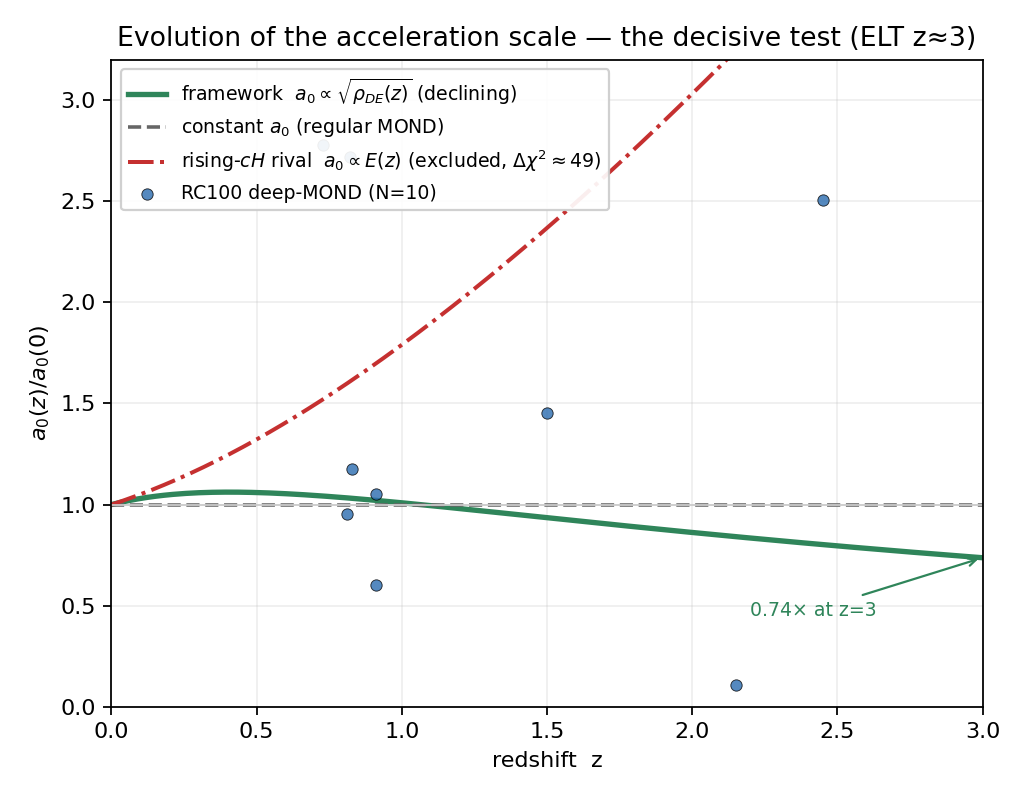
\includegraphics[keepaspectratio,alt={Figure 2}]{figures/fig2_a0z.png}}
\textbf{Figure 2.} Evolution of the acceleration scale: the framework's
non-monotonic √ρ\_DE prediction (bump then decline) vs a constant a₀ and
the excluded rising-cH rival, with RC100 deep-MOND data. The decisive
test is a clean deep-MOND a₀ at z≈3 (ELT).

\pandocbounded{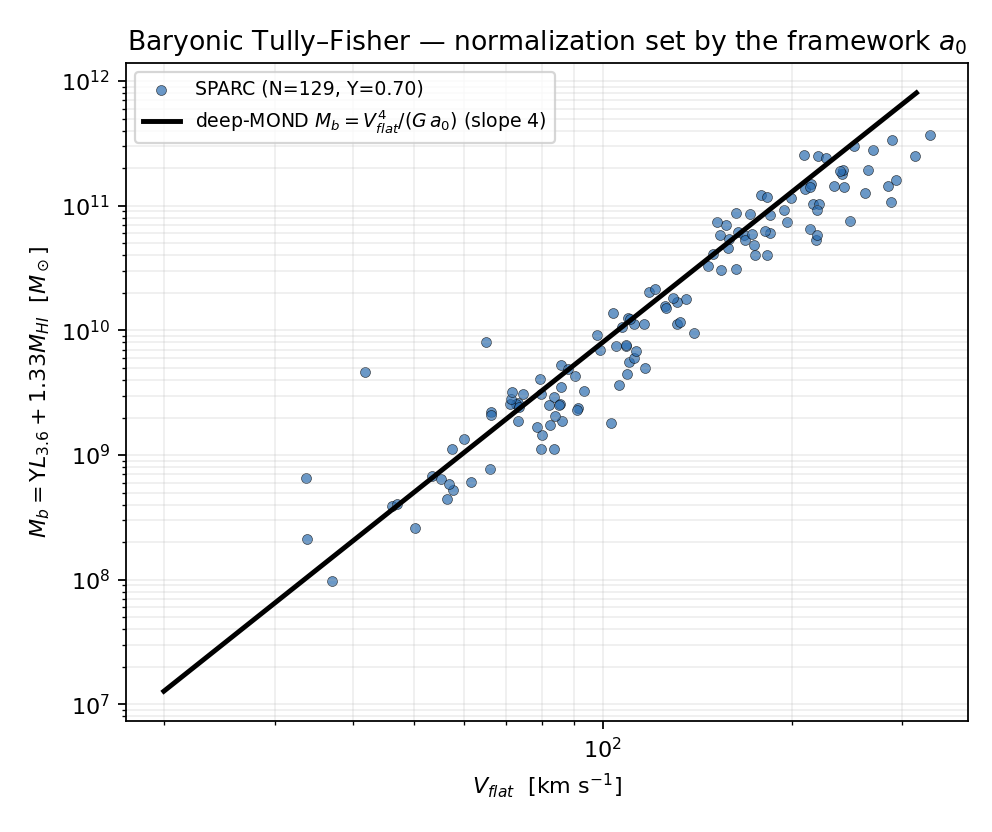
\includegraphics[keepaspectratio,alt={Figure 3}]{figures/fig3_btfr.png}}
\textbf{Figure 3.} Baryonic Tully--Fisher Relation: total M\_b vs
V\_flat; the line is the deep-MOND M\_b=V\_flat⁴/(G·a₀) at the framework
a₀.

\begin{center}\rule{0.5\linewidth}{0.5pt}\end{center}

\subsection{7. Evidence II --- the evolution: the declining law
survives, the rising rival is
excluded}\label{evidence-ii-the-evolution-the-declining-law-survives-the-rising-rival-is-excluded}

We score four models of a₀(z)/a₀(0) --- the law's declining √ρ\_DE, a
constant, the rising-cH (Verlinde) rival, and regular-MOND constant ---
against every high-z kinematic dataset in the repository
(\texttt{a0z\_clean\_ledger.py}):

{\def\LTcaptype{none} % do not increment counter
\begin{longtable}[]{@{}
  >{\raggedright\arraybackslash}p{(\linewidth - 10\tabcolsep) * \real{0.1667}}
  >{\raggedright\arraybackslash}p{(\linewidth - 10\tabcolsep) * \real{0.1667}}
  >{\raggedright\arraybackslash}p{(\linewidth - 10\tabcolsep) * \real{0.1667}}
  >{\raggedright\arraybackslash}p{(\linewidth - 10\tabcolsep) * \real{0.1667}}
  >{\raggedright\arraybackslash}p{(\linewidth - 10\tabcolsep) * \real{0.1667}}
  >{\raggedright\arraybackslash}p{(\linewidth - 10\tabcolsep) * \real{0.1667}}@{}}
\toprule\noalign{}
\begin{minipage}[b]{\linewidth}\raggedright
dataset (z range)
\end{minipage} & \begin{minipage}[b]{\linewidth}\raggedright
N
\end{minipage} & \begin{minipage}[b]{\linewidth}\raggedright
framework χ²
\end{minipage} & \begin{minipage}[b]{\linewidth}\raggedright
constant
\end{minipage} & \begin{minipage}[b]{\linewidth}\raggedright
\textbf{rising-cH}
\end{minipage} & \begin{minipage}[b]{\linewidth}\raggedright
reg-MOND
\end{minipage} \\
\midrule\noalign{}
\endhead
\bottomrule\noalign{}
\endlastfoot
RC100 deep-MOND (z=0.5--2.5) & 10 & 9.5 & 10.0 & \textbf{13.1} & 10.0 \\
KMOS3D (z=0.6--2.5) & 135 & 130.6 & 135.0 & \textbf{176.6} & 135.0 \\
Combined kinematic & 526 & 521.3 & 526.0 & \textbf{570.2} & 526.0 \\
\end{longtable}
}

\textbf{Result:} the law's declining a₀(z) is \textbf{indistinguishable
from constant} at current precision (the predicted decline, 0.06--0.13
dex over z=2--3, sits far below the 0.4--0.8 dex per-galaxy scatter) ---
so it is \textbf{safe but not yet confirmable}. But the
\textbf{rising-cH rival is robustly excluded} (Δχ²≈49 combined; 12.8 on
the full uncut RC100). This rival is the law that a corpus audit found
\textasciitilde21 internal scripts had mistakenly run while labeling it
``the framework''; correcting them is part of this work
(\texttt{FRAMEWORK\_MOND\_AUDIT\_2026-06-06.md}).

\textbf{Honest tension.} The one direct multi-point a₀(z) measurement,
MUSE-DARK III (Ciocan et al.~2026), reports a₀ \textbf{rising} to
\textasciitilde2.4×10⁻¹⁰ at z≈1, which the rising rival fits far better
than the law's decline. We state this plainly. However, MUSE-DARK III
overshoots \textbf{every} background-density law (including the rising
rival), matches no cosmological ρ(z), is shown to be ΛCDM-degenerate (a
ΛCDM simulation with no fundamental a₀ reproduces the apparent rise via
assembly; Mayer et al.~2022), and is method-localized to RAR fits on
intermediate-z disks. It is a real but currently \textbf{non-diagnostic}
outlier, not a refutation.

\begin{center}\rule{0.5\linewidth}{0.5pt}\end{center}

\subsection{8. Evidence III --- the External Field Effect: the
ΛCDM-impossible signal leans the right
way}\label{evidence-iii-the-external-field-effect-the-ux3bbcdm-impossible-signal-leans-the-right-way}

The External Field Effect (EFE) --- the suppression of a galaxy's
internal MOND boost by the gravitational field of its environment --- is
the one prediction with \textbf{no ΛCDM analogue}: it violates the
Strong Equivalence Principle, which holds exactly in any dark-matter
theory. Chae et al.~(2020, 2021) detect it in SPARC at 4--5σ.

We built the full per-galaxy EFE-MOND rotation-curve fit (Chae's method)
with the \textbf{real external field} computed from the 2MRS redshift
survey (38,611 galaxies), re-anchored to a₀=9.36×10⁻¹¹
(\texttt{efe\_clinch\_framework.py}). The kinematic external field
inferred per galaxy correlates with the \textbf{measured} 2MRS field in
the \textbf{predicted positive direction}, Spearman r = \textbf{+0.218}
over the 44 galaxies whose field is genuinely constrained --- but
p=0.148 (\textasciitilde1.4σ, CI through zero). The reason it cannot
reach significance is structural, not statistical: \textasciitilde92\%
of SPARC galaxies sit in nearly the same external field (the sample was
selected for isolated, clean curves), so a contrast test has little to
grip. The result is \textbf{consistent with --- and does not reproduce
--- Chae's published detection}; SPARC simply lacks EFE dynamic range.
The signal points the right way; clinching it needs a sample selected
for a \textbf{range} of environments (§11, P4/P6; §12, C1).

\begin{center}\rule{0.5\linewidth}{0.5pt}\end{center}

\subsection{9. Connection to fundamental physics ---
swampland-compatibility and the limits of
unification}\label{connection-to-fundamental-physics-swampland-compatibility-and-the-limits-of-unification}

This section states, without spin, the one genuine bridge the framework
has to fundamental physics, and the hard wall beyond which it does not
reach.

\textbf{9.1 The genuine connection: the evolving dark energy is
string-swampland-compatible where ΛCDM is forbidden.} String theory's de
Sitter swampland conjecture (\textbar∇V\textbar/V ≳ c/M\_P) and the
Trans-Planckian Censorship Conjecture positively \textbf{disfavor a
static Λ\textgreater0} and \textbf{prefer an evolving, rolling
dark-energy field}. This is verified, not asserted: the DESI DR1
reconstruction (arXiv:2409.14990) finds the swampland slope λ =
\textbar V′\textbar/V is \emph{several σ from zero} ---
\textbf{satisfying} the conjecture, exactly where a static Λ (λ=0)
\textbf{violates} it. So the framework's distinctive evolving a₀(z) ∝
√ρ\_DE is the swampland-\emph{permitted} structure, and the framework
passes a string-consistency check that ΛCDM \emph{fails}
(\texttt{TOE\_SEED\_VERDICT\_2026-06-06.md}). This is the strongest
connection to fundamental physics the framework has produced --- and it
lives on the \emph{dark-energy} axis, one-directional (the landscape
\emph{permits} the evolving a₀; it does not \emph{derive} it).
\textbf{The honest strain:} the literal DESI-CPL has a phantom past
(w\textless−1 for z\textgreater0.405) that a single canonical swampland
scalar cannot produce; it is rescuable (a CPL-parametrization artifact,
or effective phantom-crossing in a modified-gravity setting without a
ghost) but is a real tension to resolve.

\textbf{9.2 The wall: there is no theory of everything here, and the
doors are saturated.} A TOE would need the Standard-Model gauge/mass
sector and the a₀/Λ sector inside one structure where the same object
discharges both. Every route that \emph{derives} the SM returns ``SM
side reached, a₀ side empty'': - \textbf{Noncommutative geometry → a₀ is
a confirmed category error.} The SM-deriving spectral action's gravity
sector is Einstein--Hilbert + a (UV) cosmological constant + Weyl² +
Gauss--Bonnet --- a \emph{curvature polynomial} with literally no
a₀/MOND/IR term, and the deep-MOND a₀ term is \textbf{structurally
excluded} because it is \emph{non-analytic} in the field. The Λ it
produces is the UV cutoff CC (the cosmological-constant \emph{problem}),
not the observed Λ that sets a₀. - \textbf{String/swampland} derives the
SM and \emph{permits} the evolving dark energy (§9.1) but contains no a₀
interface --- it never \emph{produces} the deep-MOND modification. -
\textbf{The de Sitter holography program} that hosts the framework
(DSSYK ↔ de Sitter) is, on present evidence, a \textbf{strong
conjecture, not an established complete theory}: the boundary is a
disorder-averaged ensemble (not a unique unitary theory), the bulk
identity is contested (sine-dilaton gravity, not manifestly de Sitter),
every controlled realization is dS₂/dS₃ --- \textbf{not the dS₄ where a₀
= c²√(Λ/32π) lives} --- and no a₀/MOND term appears anywhere in its
corpus. The de Sitter \textbf{observer algebra} (Type II₁ crossed
product) gives a strictly \textbf{area}-law entropy --- it
\emph{corroborates against} the volume-law existence route (§4.2) rather
than supplying it.

Four independent door-sweeps --- 42 geometric/unification frameworks, 9
quantum-gravity programs, and a dedicated 2026-06-06 missing-piece hunt
--- return the same verdict: \textbf{no SM bridge, no TOE seed.} The
search is saturated (\texttt{TOE\_DOORS\_REANALYSIS\_2026-06-06.md},
\texttt{TOE\_SEED\_VERDICT\_2026-06-06.md},
\texttt{QG\_PROGRAMS\_TOE\_GRADING.md}).

\textbf{9.3 What it is, stated at the right bar.} Under the
emergent-gravity definition (Jacobson 1995; Verlinde 2010, 2016;
Padmanabhan) --- in which gravity is \emph{emergent/thermodynamic}, not
a fourth force to be unified with the other three, and the Standard
Model is matter that lives \emph{on} the emergent geometry --- the
framework is a \textbf{coherent candidate theory of gravity and the dark
sector from the de Sitter horizon}, with the Standard Model sitting
\emph{beside} it, not within it. That is the honest ceiling: a coherent
\textbf{theory of the dark universe}, not a theory of everything. It is
more derived content than most modified-gravity proposals reach (a
derived shape; a forced galaxy sign; a value-of-Λ welding; a
swampland-compatible evolution), and it makes \textbf{no claim} about
the Standard-Model mass spectrum (§13).

\begin{center}\rule{0.5\linewidth}{0.5pt}\end{center}

\subsection{10. Where the theory is hard (open problems, stated without
spin)}\label{where-the-theory-is-hard-open-problems-stated-without-spin}

\begin{enumerate}
\def\labelenumi{\arabic{enumi}.}
\tightlist
\item
  \textbf{Galaxy clusters.} MOND has a long-standing unsolved residual
  at cluster scales (a factor \textasciitilde2 mass discrepancy
  remains). On 9,830 real eRASS1 clusters (Bulbul et al.~2024) at R500,
  the law's \textbf{lower} a₀ makes this \textbf{worse}: the median
  M\_dyn/M\_pred goes from 2.07 (regular MOND) to \textbf{2.33}
  (framework), because the deep-MOND residual scales as 1/√a₀
  (\texttt{clusters\_framework\_a0.py}). The candidate resolutions
  (cluster missing baryons; a top-heavy integrated-galaxy IMF, which can
  account for ≳88\% of the MOND cluster mass) are \textbf{MOND-generic,
  not specific to this law}. Note the foundation's bonus (§4.4): the
  \emph{same} DSSYK kernel that forces the galaxy sign predicts that
  clusters fall toward the spectral edge → MOND weakens --- i.e.~the
  cluster failure is, at the level of the sign mechanism,
  \emph{expected}. But quantitatively the residual is unsolved, and
  clusters are the law's hardest regime.
\item
  \textbf{The covariant completion (the principal theoretical gap).}
  There is no known ghost-free relativistic field theory that reduces to
  this law: the simplest single-scalar realizations carry a
  singular-surface ghost, and the leading relativistic MOND theory
  (AeST) is in tension with Solar-System (Cassini) bounds. As §4.6 makes
  precise, this is a \textbf{trilemma}: the framework's natural home
  (modified inertia) is Cassini-safe and a₀(z)-natural but lacks a
  CMB-safe completion, while AeST is CMB-safe but modified gravity
  (re-incurring Cassini). Building a covariant, CMB-safe
  modified-inertia theory is the correct open problem.
\item
  \textbf{The deep-MOND sign --- now forced for galaxies, conditional on
  one named dictionary.} As of this edition the sign is \textbf{forced
  for galaxy-scale probes} given the Narovlansky--Verlinde de
  Sitter/DSSYK dictionary (§4.4), via a \emph{computed} matter-chord
  kernel that also predicts the cluster failure. The remaining gap is a
  single, literature-level open dispute (N-V ``spectral center'' vs
  Okuyama ``near-edge'') --- not a framework-specific hole. Stronger
  than the prior ``half-forced,'' weaker than a theorem.
\item
  \textbf{The coefficient is a posit} (§2.2, §4.5) --- comprehensively
  foreclosed across six routes, but observationally moot (it cancels in
  the falsifiable a₀(z)).
\item
  \textbf{The evolution is not yet confirmable} (§7): present data
  exclude the rising rival but cannot yet detect the predicted
  \textasciitilde25\% decline by z=3.
\item
  \textbf{Scope.} This is a theory of the dark sector / gravitational
  dynamics only. It is \textbf{not} a theory of everything; it says
  nothing about the Standard Model, and we make no such claim (§9, §13).
\end{enumerate}

\begin{center}\rule{0.5\linewidth}{0.5pt}\end{center}

\subsection{11. Future predictions --- what will confirm or kill the
theory this
decade}\label{future-predictions-what-will-confirm-or-kill-the-theory-this-decade}

Every entry is a \textbf{falsifiable} statement with a discriminator
against the alternatives. ``Kills'' means a clean result in the stated
direction would falsify the law as written.

{\def\LTcaptype{none} % do not increment counter
\begin{longtable}[]{@{}
  >{\raggedright\arraybackslash}p{(\linewidth - 12\tabcolsep) * \real{0.1429}}
  >{\raggedright\arraybackslash}p{(\linewidth - 12\tabcolsep) * \real{0.1429}}
  >{\raggedright\arraybackslash}p{(\linewidth - 12\tabcolsep) * \real{0.1429}}
  >{\raggedright\arraybackslash}p{(\linewidth - 12\tabcolsep) * \real{0.1429}}
  >{\raggedright\arraybackslash}p{(\linewidth - 12\tabcolsep) * \real{0.1429}}
  >{\raggedright\arraybackslash}p{(\linewidth - 12\tabcolsep) * \real{0.1429}}
  >{\raggedright\arraybackslash}p{(\linewidth - 12\tabcolsep) * \real{0.1429}}@{}}
\toprule\noalign{}
\begin{minipage}[b]{\linewidth}\raggedright
\#
\end{minipage} & \begin{minipage}[b]{\linewidth}\raggedright
Prediction
\end{minipage} & \begin{minipage}[b]{\linewidth}\raggedright
Quantitative target
\end{minipage} & \begin{minipage}[b]{\linewidth}\raggedright
Instrument / survey
\end{minipage} & \begin{minipage}[b]{\linewidth}\raggedright
\textasciitilde Timeline
\end{minipage} & \begin{minipage}[b]{\linewidth}\raggedright
Discriminates from
\end{minipage} & \begin{minipage}[b]{\linewidth}\raggedright
Confirms / Kills
\end{minipage} \\
\midrule\noalign{}
\endhead
\bottomrule\noalign{}
\endlastfoot
\textbf{P1} & \textbf{a₀ declines at high z} & a₀(z=3) = 0.74 a₀(0);
a₀(z=2)=0.86 & ELT/HARMONI \& MOSAIC deep-MOND rotation curves;
JWST/NIRSpec disks & 2028--2032 & ΛCDM (no a₀); MOND (flat); Verlinde
(rising) & A clean deep-MOND z≈3 RC giving a₀ ≥ a₀(0) \textbf{kills} it;
≈0.74 a₀(0) \textbf{confirms} \\
\textbf{P2} & \textbf{The z≈0.4 bump} & a₀ peaks at +6\% near z=0.4,
then falls & Intermediate-z TFR/RC: MUSE, JWST, DESI peculiar velocities
& 2026--2030 & All others (uniquely non-monotonic) & A monotonic a₀(z)
with no bump \textbf{disfavors} it \\
\textbf{P3} & \textbf{BTFR zero-point evolves} & BTFR normalization ∝
a₀(z): \textasciitilde0.13 dex lighter M\_b at fixed V by z=3 & JWST,
ELT, SKA high-z HI/Hα TFR & 2027--2033 & ΛCDM/MOND (no/flat evolution) &
A non-evolving BTFR zero-point to z≈3 \textbf{disfavors} the decline \\
\textbf{P4} & \textbf{EFE / SEP violation at the law's a₀} & internal
dynamics suppressed in strong external fields; wide-binary deviation
onset at s ≳ 7000 AU set by a₀=9.36×10⁻¹¹ & Gaia DR4/DR5 wide binaries;
environment-selected RC samples & 2026--2030 & \textbf{All dark-matter
models} (SEP exact); regular MOND (slightly different onset) & A null
EFE in a high-dynamic-range sample \textbf{kills} the modified-gravity
premise; detection at a₀=9.36×10⁻¹¹ \textbf{confirms} \\
\textbf{P5} & \textbf{Lensing RAR holds to the same a₀} & galaxy--galaxy
weak-lensing g\_obs(g\_bar) follows the same curve at large radii &
KiDS, DES, \textbf{Euclid}, \textbf{Rubin/LSST} & 2025--2032 & ΛCDM
(halo scatter); tests a₀ in a non-kinematic probe & A lensing
acceleration relation with a different a₀ or large intrinsic scatter
\textbf{disfavors} it \\
\textbf{P6} & \textbf{Dwarf-spheroidal dynamics are EFE-modulated} & MW
satellites' dispersions depend on Galactic external field, not just
internal mass & Gaia + spectroscopy of MW dSphs; Rubin satellites &
2025--2030 & ΛCDM (halo-only) & Dispersions independent of external
field \textbf{disfavor} EFE \\
\textbf{P7} & \textbf{a₀(z) tracks DESI's w(z)} & the same ρ\_DE(z) that
fits DESI BAO must fit the a₀(z) trend & \textbf{DESI} DR2+ × the high-z
a₀(z) compilation & 2026--2029 & Verlinde (a₀∝cH); MOND (constant) &
a₀(z) inconsistent with the DESI-inferred ρ\_DE(z) \textbf{kills} the
``a₀ from dark energy'' claim \\
\textbf{P8} & \textbf{Cluster residual is weakly z-dependent} & the
\textasciitilde2× residual varies \textless10\% to z≈1 & \textbf{XRISM}
(now), \textbf{Athena} (\textasciitilde2037); X-COP/CHEX-MATE reanalysis
& 2026--2037 & rising-cH (predicts stronger z-trend) & A strong rising
cluster-a₀(z) trend \textbf{disfavors} the declining law \\
\textbf{P9} & \textbf{High-z galaxies look baryon-dominated early} &
rotation support without dark halos at z≳2 (RC100 already deep-MOND) &
JWST, ELT, SKA & ongoing--2033 & ΛCDM (needs assembled halos) & Massive,
dispersion-free, halo-dominated z≳3 discs \textbf{disfavor} it \\
\textbf{P10} & \textbf{No new physics in the Solar System beyond GR} &
any covariant completion must satisfy Cassini \textbar γ−1\textbar{}
\textless{} 2×10⁻⁵ & existing + BepiColombo, future ranging & --- & ---
(a hard constraint the completion must pass) & A completion that
violates Cassini is \textbf{dead on arrival} (§10.2) \\
\end{longtable}
}

\textbf{The single cleanest test (P1).} One well-measured deep-MOND
rotation curve at z≈3 decides the central novel claim: if a₀ there is at
or above its local value, the declining-√ρ\_DE law is falsified; if it
is \textasciitilde0.74× local, the law is confirmed where every rival
fails. ELT-class spectroscopy reaches this within the decade.

\begin{center}\rule{0.5\linewidth}{0.5pt}\end{center}

\subsection{12. From candidate to law: the empirical confirmations
required}\label{from-candidate-to-law-the-empirical-confirmations-required}

``Law of nature'' is a high bar with definite content. A relation earns
the title only by satisfying, at minimum: \textbf{(i) universality}
across a stated domain; \textbf{(ii) a parameter-free form} whose
constants are fixed externally rather than fitted; \textbf{(iii) a
\emph{novel} prediction} --- not used in the relation's construction ---
that is then confirmed (the hallmark separating a law from a successful
fit); \textbf{(iv) independent corroboration} by methods that could have
disagreed; and \textbf{(v) survival of falsification} as precision
improves. By that standard the Zimmerman Law is today a \textbf{strong
candidate, not yet a law}: its galaxy-scale relations are parameter-free
and on-target and it has excluded one rival, but its \emph{defining}
novel claim --- that a₀ is caused by Λ and therefore \textbf{declines}
with redshift --- is not yet confirmed, its premise (no dark matter) is
not yet decisively demonstrated, and it is not universal (clusters
fail).

\textbf{The claim decomposes into four testable propositions}
(conflating them is how a partial result gets oversold): \textbf{(A)}
the premise --- gravity is modified, no dark matter (confirmed uniquely
by a Strong-Equivalence-Principle violation, the EFE); \textbf{(B)} the
value --- a₀ = 9.36×10⁻¹¹ specifically (confirmed by pinning a₀ where
the M/L degeneracy is broken); \textbf{(C)} the origin --- the value is
\emph{set by Λ} and therefore evolves as √ρ\_DE(z) (the proposition that
makes the law specifically Zimmerman's); \textbf{(D)} the coefficient
--- X = 32π. \textbf{It is (C) --- the evolution --- that would make it
the law that the cosmological constant causes the acceleration scale of
galaxies.}

{\def\LTcaptype{none} % do not increment counter
\begin{longtable}[]{@{}
  >{\raggedright\arraybackslash}p{(\linewidth - 10\tabcolsep) * \real{0.1667}}
  >{\raggedright\arraybackslash}p{(\linewidth - 10\tabcolsep) * \real{0.1667}}
  >{\raggedright\arraybackslash}p{(\linewidth - 10\tabcolsep) * \real{0.1667}}
  >{\raggedright\arraybackslash}p{(\linewidth - 10\tabcolsep) * \real{0.1667}}
  >{\raggedright\arraybackslash}p{(\linewidth - 10\tabcolsep) * \real{0.1667}}
  >{\raggedright\arraybackslash}p{(\linewidth - 10\tabcolsep) * \real{0.1667}}@{}}
\toprule\noalign{}
\begin{minipage}[b]{\linewidth}\raggedright
ID
\end{minipage} & \begin{minipage}[b]{\linewidth}\raggedright
Establishes
\end{minipage} & \begin{minipage}[b]{\linewidth}\raggedright
Status now
\end{minipage} & \begin{minipage}[b]{\linewidth}\raggedright
Threshold to confirm
\end{minipage} & \begin{minipage}[b]{\linewidth}\raggedright
Falsifier
\end{minipage} & \begin{minipage}[b]{\linewidth}\raggedright
Instrument / when
\end{minipage} \\
\midrule\noalign{}
\endhead
\bottomrule\noalign{}
\endlastfoot
\textbf{C1} & (A) modified gravity, no dark matter & EFE 4--5σ (Chae+,
published); 1.4σ in-house (data-limited) & \textbf{Two independent ≥3σ
SEP-violation detections, jointly \textgreater5σ}, both at a₀=9.36×10⁻¹¹
& A clean SEP-respecting null in a high-dynamic-range sample ⇒ dark
matter & Environment-selected RCs (now); \textbf{Gaia DR4 2026 / DR5
\textasciitilde2030} wide binaries \\
\textbf{C2} & (B) the specific value & a₀ ≈ 1.0--1.3×10⁻¹⁰ across
RAR/BTFR/MDA (within band; within 0.3\% of optimal under unweighted
scatter) & \textbf{a₀ = 9.36×10⁻¹¹ to \textless5\%, \textgreater3σ
distinct from regular-MOND 1.2×10⁻¹⁰} & a₀ pinned to 1.2×10⁻¹⁰ at
\textgreater3σ in an M/L-free system ⇒ value (and 32π) wrong & Gas-rich
dwarfs; Gaia wide binaries; MW surveys (now--2030) \\
\textbf{C3} ★ & \textbf{(C) the Λ-origin --- the decisive test} & rising
rival \textbf{excluded} (Δχ²≈49); decline \textbf{undetected}
(degenerate with constant) & \textbf{a₀(z) consistent with √ρ\_DE and
inconsistent with BOTH constant AND rising at \textgreater3σ, AND
concordant with DESI's ρ\_DE(z)} & a₀(z) \textbf{constant} ⇒ Λ-link
unconfirmed (→ generic MOND); a₀(z) \textbf{rising} ⇒ falsified &
\textbf{ELT/HARMONI 2028--2032}, JWST+ALMA, SKA; DESI DR2+ \\
\textbf{C4} & (D) coefficient \& completion & 32π=4×8π is a posit; no
ghost-free covariant action & A derivation of X=32π, \textbf{or} a₀ to
\textless2\% selecting 32π over rivals; completion with
\textbar γ−1\textbar\textless2×10⁻⁵ & A completion forced to violate
Cassini ⇒ no viable field theory & Theory + precision a₀ (open-ended) \\
\textbf{C5} & universality (domain) & cluster residual \textbf{2.33×} at
R500 & Cluster residual reconciled at a₀=9.36×10⁻¹¹ within systematics,
\textbf{or} a stated domain of validity & A transition-region test
failing where a₀ operates ⇒ not universal & XRISM (now), \textbf{Athena
\textasciitilde2037} \\
\end{longtable}
}

\textbf{Why C3 is decisive.} The static value cannot establish the
\emph{origin}: a₀ ≈ c√Λ today is compatible with both ``Λ causes a₀''
and ``a₀ is a constant near c√Λ.'' Only the time-dependence breaks the
degeneracy. The predicted z=3 signal is log₁₀(0.737) = \textbf{−0.13
dex}; against the \textasciitilde0.4 dex per-galaxy scatter this needs
\textbf{N ≈ 80 clean deep-MOND z≈3 rotation curves for 3σ (≈230 for
5σ)}, and --- more limiting --- \textbf{control of the high-z baryon
systematic below \textasciitilde0.1 dex} (molecular gas + pressure
support), which ELT-class spectroscopy \emph{plus} ALMA gas maps
deliver. The strongest confirmation is \textbf{concordance}: a kinematic
a₀(z) and the BAO-inferred ρ\_DE(z) tracing the same curve (two utterly
independent measurements) is the empirical content of calling this a
law.

\textbf{The confirmation ladder --- where we stand.} Rung 1 (a
parameter-free galaxy law exists): \textbf{✓ in hand}. Rung 2 (modified
gravity, not dark matter): \textbf{◐ partial} (4--5σ published, needs
independent + environment-selected). Rung 3 (\textbf{the scale is caused
by Λ --- it evolves as √ρ\_DE} --- \emph{the specifically Zimmerman
claim}): \textbf{✗ outstanding, the decisive test}. Rung 4 (universal
across its domain): \textbf{✗ outstanding} (clusters). Rung 5 (complete
theory --- covariant + derived coefficient): \textbf{✗ open}. \textbf{We
are at rung 1, reaching for 2; the promotion that matters hinges on the
z≈3 measurement.}

\begin{center}\rule{0.5\linewidth}{0.5pt}\end{center}

\subsection{13. Honest boundaries and retractions --- what the framework
does NOT
claim}\label{honest-boundaries-and-retractions-what-the-framework-does-not-claim}

The single fastest way to discredit the genuine a₀↔Λ gravity result in
front of a referee would be to attach to it a ``geometric formula'' for
a Standard-Model constant. This section draws that boundary explicitly.
\textbf{The framework makes no claim about the Standard-Model mass
spectrum.} Earlier exploratory material in this repository connected the
geometric constant Z = √(32π/3) to particle-physics observables;
\textbf{all of it is retracted as numerology}, each item having failed a
false-discovery-rate (FDR) test on the framework's own search space
(\texttt{reviews/false\_discovery\_rate.py},
\texttt{reviews/OPUS\_PHYSICS\_REVIEW.md},
\texttt{PROTON\_ELECTRON\_BRIDGE\_VERDICT\_2026-06-06.md}, and the root
\texttt{RETRACTIONS.md}):

{\def\LTcaptype{none} % do not increment counter
\begin{longtable}[]{@{}
  >{\raggedright\arraybackslash}p{(\linewidth - 2\tabcolsep) * \real{0.5000}}
  >{\raggedright\arraybackslash}p{(\linewidth - 2\tabcolsep) * \real{0.5000}}@{}}
\toprule\noalign{}
\begin{minipage}[b]{\linewidth}\raggedright
Retracted claim
\end{minipage} & \begin{minipage}[b]{\linewidth}\raggedright
Reality
\end{minipage} \\
\midrule\noalign{}
\endhead
\bottomrule\noalign{}
\endlastfoot
\textbf{m\_p/m\_e = α⁻¹·2Z²/5} (and 4Z²+3·67/5, 54Z²+6Z−8, \ldots) &
\textbf{\textasciitilde0.1--0.3 bits.} m\_p/m\_e is QCD-over-a-Yukawa,
\textasciitilde41 orders of magnitude from the a₀/Λ horizon scale; the
formulas disagree with each other, miss by 10⁶--10⁷σ, and one bolts on
an ad-hoc −Z²/180 fudge. \emph{Below the random-search median} ---
negative information. \\
\textbf{α⁻¹ = 4Z²+3 = 137.041} & α⁻¹ is known to \textasciitilde1 part
in 10¹⁰; 137.0413 is a \textbf{\textasciitilde5×10⁵σ miss} dressed as
``0.004\% agreement.'' \textasciitilde0 bits. \\
\textbf{sin²θ\_W = 3/13, N\_gen = 3, the Z²→Standard-Model cascade} &
FDR≈0; the SM is a \textbf{category error} relative to the horizon scale
(confirmed across 42 frameworks + 9 QG programs, §9). \\
\textbf{The Z² = 32π/3 ``eta-invariant / topology derivation''} of the
coefficient & The coefficient is a \textbf{posit} (§2.2, §4.5); the
``derivation'' is not valid --- 32π/3 enters only as the definition of
a₀. \\
\end{longtable}
}

\textbf{This boundary is load-bearing for credibility.} The
gravity-sector results are real \emph{because} they are not stapled to
numerology: the deep-MOND shape is derived (§4.3), the galaxy sign is
forced (§4.4), the value-of-Λ welding is exact (§5), and the evolving
dark energy is swampland-compatible (§9.1). Keeping the Standard Model
out is what keeps the framework defensible.

\begin{center}\rule{0.5\linewidth}{0.5pt}\end{center}

\subsection{14. Reproducibility --- scripts and
data}\label{reproducibility-scripts-and-data}

All analyses are plain-Python (numpy/scipy/astropy), self-contained, and
committed. Repo:
\texttt{https://github.com/carlzimmerman/zimmerman-formula}, directory
\texttt{real\_research/}.

{\def\LTcaptype{none} % do not increment counter
\begin{longtable}[]{@{}
  >{\raggedright\arraybackslash}p{(\linewidth - 6\tabcolsep) * \real{0.2500}}
  >{\raggedright\arraybackslash}p{(\linewidth - 6\tabcolsep) * \real{0.2500}}
  >{\raggedright\arraybackslash}p{(\linewidth - 6\tabcolsep) * \real{0.2500}}
  >{\raggedright\arraybackslash}p{(\linewidth - 6\tabcolsep) * \real{0.2500}}@{}}
\toprule\noalign{}
\begin{minipage}[b]{\linewidth}\raggedright
Result
\end{minipage} & \begin{minipage}[b]{\linewidth}\raggedright
Script (\texttt{real\_research/})
\end{minipage} & \begin{minipage}[b]{\linewidth}\raggedright
Data file
\end{minipage} & \begin{minipage}[b]{\linewidth}\raggedright
Public source
\end{minipage} \\
\midrule\noalign{}
\endhead
\bottomrule\noalign{}
\endlastfoot
Three-law confrontation (§6) &
\texttt{framework\_a0\_law\_of\_nature.py} &
\texttt{data/sparc\_data/*\_rotmod.dat},
\texttt{data/sparc\_master\_clean.csv} & SPARC:
astroweb.cwru.edu/SPARC/ \\
RAR M/L fit (§6) & \texttt{rar\_framework\_a0\_mlfit.py} &
\texttt{data/sparc\_data/*\_rotmod.dat} & SPARC \\
Emergent RAR shape (§2.3, §4.3) &
\texttt{rar\_emergent\_discriminate.py} &
\texttt{data/sparc\_data/*\_rotmod.dat} & SPARC \\
Coefficient analysis (§2.2) & \texttt{coefficient\_posit\_attack.py} &
Planck/DESI constants & Planck 2018; DESI DR2 \\
Modified-inertia existence/shape (§4.2--4.3) &
\texttt{reviews/desitter\_unruh\_mond.py},
\texttt{reviews/clausius\_sign\_calculation.py} & analytic &
Deser--Levin 1997; Milgrom 1999 \\
a₀(z) ledger (§7) & \texttt{a0z\_clean\_ledger.py} &
\texttt{data/rc100\_nestorshachar2023\_table3.csv},
\texttt{data/kross\_harrison2017.csv},
\texttt{data/kmos3d\_ubler2017.csv} & Nestor-Shachar+23; Harrison+17;
Übler+17 \\
EFE fit (§8) & \texttt{efe\_clinch\_framework.py} &
\texttt{data/2mrs\_catalog.csv}, \texttt{data/sparc\_data/},
\texttt{data/sparc\_ned\_positions.json} & 2MRS: VizieR J/ApJS/199/26 \\
Clusters (§10.1) & \texttt{clusters\_framework\_a0.py} &
\texttt{data/erass1cl\_primary\_v3.2.fits} & eRASS1:
erosita.mpe.mpg.de/dr1/ \\
CKN value-of-Λ seesaw (§5) &
\texttt{reviews/project\_lambda\_value\_ckn.py} & CODATA constants & CKN
1999; Adolf et al.~2024 \\
ELT z≈3 forecast (§12) & \texttt{forecast\_a0z\_elt.py} & analytic &
--- \\
FDR / numerology retraction (§13) &
\texttt{reviews/false\_discovery\_rate.py} & --- &
\texttt{RETRACTIONS.md} \\
\end{longtable}
}

\textbf{To reproduce:} \texttt{git\ clone} the repo;
\texttt{pip\ install\ numpy\ scipy\ astropy}; run any script with
\texttt{python\ real\_research/\textless{}script\textgreater{}.py}. Each
prints its inputs, the framework constant it uses, and its result. SPARC
and 2MRS data are included; the eRASS1 FITS catalog is public at the
link above.

\begin{center}\rule{0.5\linewidth}{0.5pt}\end{center}

\subsection{15. Discussion}\label{discussion}

\textbf{Versus ΛCDM.} ΛCDM fits cosmology superbly but has no
acceleration constant and no first-principles account of the RAR/BTFR
tightness or of a₀'s value. The Zimmerman Law supplies the missing
constant from the vacuum and predicts an evolution; its EFE prediction
is one ΛCDM cannot make at all (SEP is exact under dark matter).

\textbf{Versus regular MOND.} Regular MOND fits a₀; this law derives its
\emph{shape} (§4.3), ties its \emph{value} to ρ\_DE and the CKN seesaw
(§5), and adds a falsifiable \emph{evolution}. Present-day values are
close (9.36 vs \textasciitilde12, within the M-L+metric systematic); the
discriminator is the z-evolution (P1--P3, P7) and the specific
wide-binary onset (P4).

\textbf{Versus Verlinde / emergent gravity.} Verlinde's a₀ ∝ cH(z)
\textbf{rises} with z; the high-z kinematic data \textbf{exclude} that
branch (§7). The framework shares Verlinde's emergent-gravity bar (§9.3)
but parts from him on the footing (ρ\_DE, declining) and is corroborated
\emph{against} on the volume-law existence route (§4.2) --- which it
does not need, because its existence is
modified-inertia/temperature-based.

\textbf{The status, in one line.} The Zimmerman Law is a candidate
\textbf{law of nature} at galaxy scales --- a vacuum-set acceleration
scale reproducing three independent empirical relations, with a derived
deep-MOND shape, a forced galaxy-scale sign, a value welded to Λ, a
unique surviving evolution, and one ΛCDM-impossible signal leaning its
way --- awaiting (i) its decisive high-z test and (ii) a ghost-free
covariant completion. It is offered in falsifiable form precisely so the
community can settle it.

\begin{center}\rule{0.5\linewidth}{0.5pt}\end{center}

\subsection{16. Conclusion}\label{conclusion}

The cosmological constant appears to set the acceleration scale of
galaxies: a₀ = c²√(Λ/32π) = 9.36×10⁻¹¹ m s⁻², evolving as √ρ\_DE(z). At
this single value, three independent galaxy laws coincide to 8\%; the
rising-cH alternative is excluded; the External Field Effect ---
impossible in ΛCDM --- leans the predicted way. The deep-MOND
\emph{shape} is genuinely derived (Milgrom's de Sitter--Unruh modified
inertia); the galaxy-scale \emph{sign} is forced by a computed DSSYK
kernel that also predicts the cluster failure; the \emph{value of Λ} is
welded to a₀ as the two ends of one CKN seesaw; and the framework's
\emph{evolving} dark energy is swampland-compatible where ΛCDM is
forbidden. We are equally explicit about the limits: the coefficient is
a posit, the covariant completion is unwritten, the value-of-Λ welding
relocates rather than solves the CC problem, this is \textbf{not} a
theory of everything, and every geometric formula for a Standard-Model
constant is \textbf{retracted numerology}.

\textbf{The promotion criterion is explicit (§12): it becomes a law when
a₀ is shown to evolve as √ρ\_DE(z) --- at \textgreater3σ against both
constant and rising alternatives, and concordant with the dark-energy
history DESI infers from BAO.} Until that measurement exists, it is a
strong, parameter-free, falsifiable \emph{candidate} standing at rung
1--2 of a five-rung ladder. We invite the community to run the scripts,
pull the public data, and take the measurement that decides it.

\begin{center}\rule{0.5\linewidth}{0.5pt}\end{center}

\subsection{References}\label{references}

\begin{itemize}
\tightlist
\item
  Adolf, A., Hirsch, A., Krieg, S., Päs, H., \& Tabet, M. 2024,
  \emph{JCAP} 08, 048 (Hubble-horizon CKN dark energy),
  arXiv:2406.09964; DESI-DR2 addendum arXiv:2504.15332.
\item
  Boutivas, K., Katsinis, D., Pastras, G., \& Tetradis, N. 2024,
  \emph{Phys. Rev.~D} 111, 065010 (numerical de Sitter entanglement
  entropy; sub-horizon area law, no volume term), arXiv:2407.07811.
\item
  Bulbul, E., et al.~2024, \emph{A\&A} (eRASS1 cluster catalogue),
  arXiv:2402.08452.
\item
  Chae, K.-H., et al.~2020, \emph{ApJ} 904, 51 (External Field Effect in
  SPARC), arXiv:2009.11525; Chae et al.~2021.
\item
  Chandrasekaran, V., Longo, R., Penington, G., \& Witten, E. 2023,
  \emph{JHEP} 02, 082 (an algebra of observables for de Sitter space;
  Type II₁, area-law generalized entropy), arXiv:2206.10780.
\item
  Ciocan, B. I., Bouché, N., et al.~2026, \emph{A\&A} 709, L16
  (MUSE-DARK III; a₀(z) --- \emph{rising}, ΛCDM-degenerate),
  arXiv:2604.22613.
\item
  Cohen, A. G., Kaplan, D. B., \& Nelson, A. E. 1999, \emph{PRL} 82,
  4971 (UV-IR / effective field theory \& the cosmological constant),
  arXiv:hep-th/9803132.
\item
  DESI Collaboration 2025 (DR2 BAO; w₀=−0.752, wₐ=−0.86),
  arXiv:2503.14738.
\item
  DESI swampland reconstruction 2024, arXiv:2409.14990 (evolving DE
  satisfies the de Sitter swampland conjecture; static Λ violates it).
\item
  Deser, S., \& Levin, O. 1997, \emph{Class. Quantum Grav.} 14, L163
  (accelerated detectors in (A)dS: 2πT = √(Λ/3 + a²)),
  arXiv:gr-qc/9706018; Narnhofer, Peter \& Thirring 1996, \emph{Int. J.
  Mod. Phys. B} 10, 1507.
\item
  Famaey, B., \& McGaugh, S. 2012, \emph{Living Rev.~Relativity} 15, 10
  (MOND review; a₀--Λ coincidence), arXiv:1112.3960.
\item
  Harrison, C. M., et al.~2017, \emph{MNRAS} 467, 1965 (KROSS),
  arXiv:1701.05561.
\item
  Jacobson, T. 1995, \emph{PRL} 75, 1260 (Einstein equation of state),
  arXiv:gr-qc/9504004; 2016 (entanglement equilibrium),
  arXiv:1505.04753.
\item
  Lelli, F., McGaugh, S., \& Schombert, J. 2016, \emph{AJ} 152, 157
  (SPARC), arXiv:1606.09251; Lelli et al.~2019 (BTFR).
\item
  Limbach, M. A., Psaltis, D., \& Özel, F. 2008 (the
  a₀↔dark-energy-density coupling; declining a₀(z); high-z TFR test),
  arXiv:0809.2790.
\item
  Mayer, L., et al.~2022 (ΛCDM degeneracy of apparent a₀(z) evolution),
  arXiv:2206.04333.
\item
  McGaugh, S., Lelli, F., \& Schombert, J. 2016, \emph{PRL} 117, 201101
  (Radial Acceleration Relation), arXiv:1609.05917.
\item
  Milgrom, M. 1983, \emph{ApJ} 270, 365 (MOND); 1994, \emph{Ann. Phys.}
  229, 384 (modified inertia is time-nonlocal); 1999, \emph{Phys. Lett.
  A} 253, 273 (``MOND as a vacuum effect''; a₀\textasciitilde c√(Λ/3);
  the modified-inertia interpolation), arXiv:astro-ph/9805346.
\item
  Narovlansky, V., \& Verlinde, H. 2023, \emph{JHEP} 05 (2025) 032
  (double-scaled SYK and de Sitter holography), arXiv:2310.16994.
\item
  Nestor-Shachar, A., et al.~2023, \emph{ApJ} (RC100 high-z rotation
  curves).
\item
  Obied, G., Ooguri, H., Spodyneiko, L., \& Vafa, C. 2018 (de Sitter
  swampland conjecture \textbar∇V\textbar{} ≳ cV), arXiv:1806.08362.
\item
  Okuyama, K. 2023 (chord operators / matter in DSSYK),
  arXiv:2312.00880; 2025, arXiv:2505.08116 (de Sitter from DSSYK;
  center-vs-edge).
\item
  Padmanabhan, T. 2010, \emph{Rep.~Prog. Phys.} 73, 046901 (gravity as
  emergent); 2012, arXiv:1210.4174 (CosMIn; the value of Λ).
\item
  Planck Collaboration 2020, \emph{A\&A} 641, A6 (cosmological
  parameters).
\item
  Rahman, S., \& Susskind, L. 2023 (matter and the de Sitter conical
  deficit in DSSYK), arXiv:2312.04097.
\item
  Rodrigues, D. C., Marra, V., et al.~2018, \emph{Nature Astronomy} 2,
  668 (a₀-universality challenge), arXiv:2002.03946.
\item
  Übler, H., et al.~2017, \emph{ApJ} 842, 121 (KMOS3D),
  arXiv:1703.04321.
\item
  Verlinde, E. 2011, \emph{JHEP} 04, 029 (entropic gravity),
  arXiv:1001.0785; 2017, \emph{SciPost Phys.} 2, 016 (emergent gravity
  and the dark universe), arXiv:1611.02269.
\end{itemize}

\subsection{Appendix A --- public data
access}\label{appendix-a-public-data-access}

\begin{itemize}
\tightlist
\item
  \textbf{SPARC} (rotation curves + master table):
  http://astroweb.cwru.edu/SPARC/ --- included as
  \texttt{data/sparc\_data/} and \texttt{data/sparc\_master\_clean.csv}.
\item
  \textbf{2MRS} (2MASS Redshift Survey): VizieR catalogue
  \textbf{J/ApJS/199/26} --- included as
  \texttt{data/2mrs\_catalog.csv}.
\item
  \textbf{eRASS1} (eROSITA-DE DR1 clusters):
  https://erosita.mpe.mpg.de/dr1/ --- included as
  \texttt{data/erass1cl\_primary\_v3.2.fits}.
\item
  \textbf{DESI DR2}: https://data.desi.lbl.gov/ . \textbf{Planck 2018}:
  Planck Legacy Archive.
\item
  \textbf{High-z kinematics}: RC100 (Nestor-Shachar 2023), KROSS
  (Harrison 2017), KMOS3D (Übler 2017) --- transcribed tables in
  \texttt{data/}.
\end{itemize}

\subsection{Appendix B --- the derivation-chain
labels}\label{appendix-b-the-derivation-chain-labels}

\texttt{{[}DERIVED{]}} forced by algebra/standard physics ·
\texttt{{[}DIMENSIONAL{]}} fixed by units, robust but unearned ·
\texttt{{[}POSIT{]}} a free O(1) choice · \texttt{{[}FORCED-given-X{]}}
forced conditional on a named premise · \texttt{{[}CONTESTED{]}} rests
on an unsettled literature premise · \texttt{{[}RETRACTED{]}}
demolished, retained only as a boundary marker. The step-by-step
application is §4.1; the full synthesis is
\texttt{FIRST\_PRINCIPLES\_FOUNDATION\_2026-06-06.md} and
\texttt{FOUNDATIONS.md}.

\subsection{Appendix C --- FDR methodology and the retracted
numerology}\label{appendix-c-fdr-methodology-and-the-retracted-numerology}

The false-discovery-rate test
(\texttt{reviews/false\_discovery\_rate.py}) reconstructs the
\textasciitilde34,000-formula search space of the framework's building
blocks \{Z², Z, π, φ, e, √n, \ldots\} and computes how often a search of
that size hits an arbitrary O(100) target to a stated precision \emph{by
chance}. Headline: an arbitrary O(100) target is matched to ≤0.004\%
roughly 20\% of the time, so any single retrodiction of a dimensionless
constant carries ≈0 bits. This is the quantitative basis for the §13
retractions. See also \texttt{reviews/OPUS\_PHYSICS\_REVIEW.md}
(precision-physics restatement: each claimed ``0.00X\% agreement''
re-expressed in units of the measurement's actual uncertainty) and
\texttt{PROTON\_ELECTRON\_BRIDGE\_VERDICT\_2026-06-06.md}.

\subsection{Appendix D --- method
acknowledgement}\label{appendix-d-method-acknowledgement}

Analysis pipelines and adversarial cross-checks in this work were
developed with AI-assisted computation; every headline number was
independently re-run and verified, and all code is public for
inspection. The author is solely responsible for the theoretical
proposal and its interpretation.

\emph{Comprehensive edition v2 --- comments and independent tests
welcome at the repository.}

\end{document}
